
\SubCity{Kurn}
{18.000 (65\% humans, 10\% elves, 6\% muls, 6\% aarakocra, 5\% dwarves, 4\% half-elves, 3\% half-giants, 1\% other).}
{livestock, magic items, medicines.}
{Elven, Kurnan.}
{
\begin{figure*}[b!]
\centering
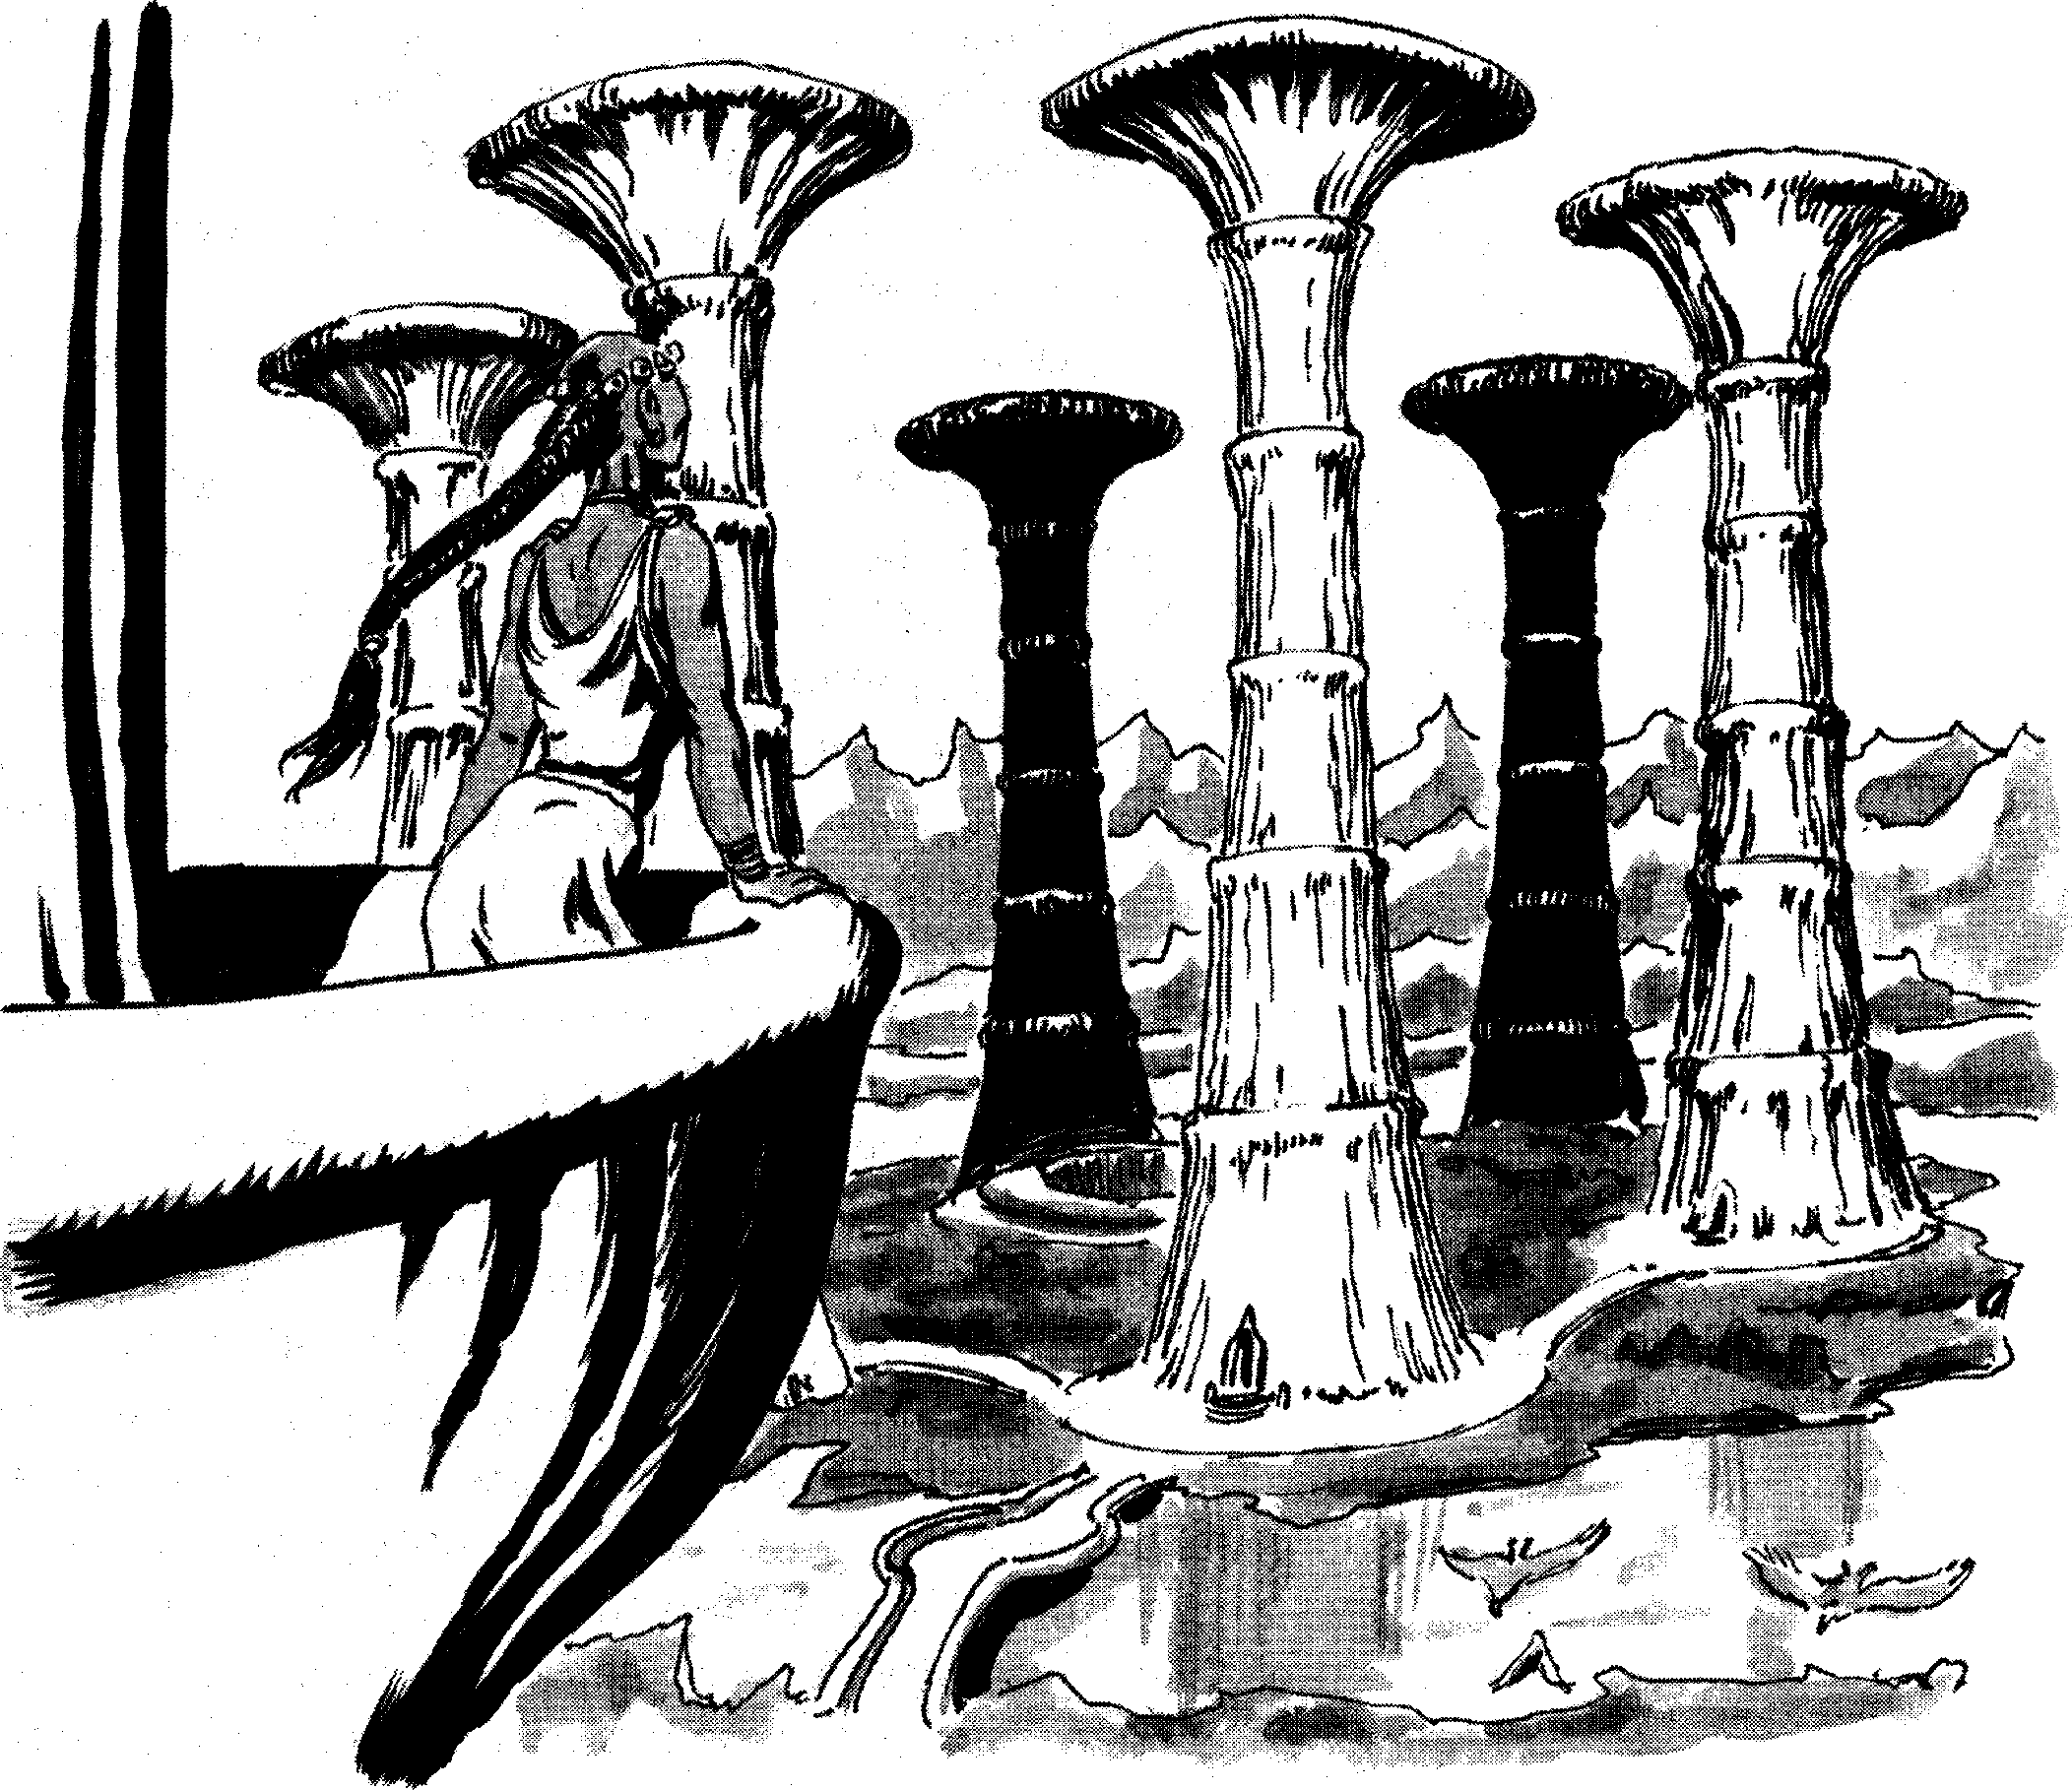
\includegraphics[height=0.4\paperheight]{images/kurn-1.png}
\WOTC
\end{figure*}
	Kurn is actually two city-states: an ancient, public metropolis, and a utopian city hidden from the rest of the world. Old Kurn sits in a lush meadow on the eastern side of the White Mountains. The trade road running north out of Draj connects Kurn to the Tyr Region, and the city welcomes merchants from the south. New Kurn lies in a fertile valley hidden among the White Mountains themselves. A secluded road protected by a towering fortress keeps the valley safe from unwanted visitors---and New Kurn doesn't want any visitors.

	Old Kurn was a prosperous but relatively small city from the Green Age that suffered great devastation in the early days of the Cleansing Wars. Once situated in a vast forest that has long since faded from the landscape, the elf city of Kurn was destroyed by the Champion called Albeorn, Slayer of Elves. When the Champions finally turned against Rajaat and became the dragon kings, the one named Keltis decided to build his city-state on the ruins of Old Kurn. He changed his name to Oronis, but decided to retain the name of the city he was building over.

	The ruins weren't in as bad a shape as Oronis originally thought. He was able to build upon many of the foundations, and a few whole structures were still fit for use. Within a decade, Oronis' Kurn was established. Within five decades, it was thriving. For five hundred years, Kurn followed the same course as the other sorcerer-king domains. Throughout that time, Oronis was troubled by something few of his peers possessed---his conscience.

	When he was Keltis, Lizard Man Executioner, he succeeded at the task Rajaat handed to him. He eliminated the entire race from the face of Athas. As the years passed and Keltis the Champion became Oronis the sorcerer-king, images of the atrocities he committed started to haunt him. After Oronis advanced to a second stage dragon king, his problems intensified. Now he had the deaths of his subjects on his head, for he had to use a specified amount of life force to power his transformation.

	He decided that none of this was what Rajaat originally promised him. Where was the restoration of the world? Athas hadn't gotten better because of the Cleansing Wars. It had gotten worse. What's more, the sorcerer-kings were continuing the downward spiral, slowly killing the world by their actions. Oronis refused to be a part of that trend any longer. He renounced his defiling skills and his status as a dragon king and sought a different path.

	That was when Kurn broke off relations with the other city-states. Mercantile activities continued, of course, but at a reduced rate. After a time, Kurn became one of the forgotten cities---just as Oronis had hoped. In the meantime, he set the next part of his plan for redemption in motion. Oronis wanted to make amends for the horrors of his past.

	The first step was to change the rules of society in Kurn. Though the city had to maintain an illusion of normalcy to keep the other sorcerer-kings from detecting treachery or weakness, Oronis secretly freed all slaves and instituted fair and just practices at all levels of society. He swore his citizens to secrecy, for if word got out he was sure his one-time peers would flock to Kurn like gith to a dying braxat. The second step was to begin construction on the utopia he envisioned. Like all ex-Champions, Oronis originally wanted to return Athas to the glory of the Blue Age.

	He decided to once more strive for that goal. In a hidden valley among the peaks of the White Mountains, the foundation stones of New Kurn were laid. As his templars and citizens worked to build New Kurn, Oronis went in search of a better path to power. Using the techniques and practices of preserving magic, Oronis looked for a way to combine magic with psionics in a more positive way than through dragon magic. It took nearly 1,000 years of study and experimentation for Oronis to develop the preserver metamorphosis spell. With it, the reformed sorcerer-king could become an advanced being aligned to goodness instead of another force for evil.

	Today, the twin cities of Kurn continue along their parallel courses. Old Kurn displays a typical sorcerer-king's domain to the other inhabitants of the region, at least on the surface, while New Kurn works to complete Oronis' experiment in regressing a small portion of Athas back through time. Between the two cities, Kurn has a total population of 18,000 people. The majority live in the new city, as each year more citizens are moved from the old city to the new. Old Kurn has such a small number of residents that it appears to be almost a ghost town, and one day Oronis plans to completely abandon it in favor of his secluded valley.
}
{
	The state of life in Kurn depends on which of the twin cities is being considered. Old Kurn, on the surface, appears to be much like any city in the Tyr Region still ruled by a sorcerer-king. Surface appearances, however, can be deceiving. Travelers who stay for any length of time might notice a few oddities. For example, the slaves seem to have a sparkle in their eyes and a bounce in their step that isn't seen in the other city-states, and templars aren't given as wide a berth as their counterparts in Urik or Nibenay. Additionally, while the merchant and tradesmen districts are always crowded, the rest of the city is as empty and desolate as the ruins of Giustenal.

	Old Kurn maintains its illusion of business-as-usual through the cooperation of its citizens and the advanced powers of its sorcerer-king. If visitors notice that the noble and templar quarters of the city are practically deserted, they usually attribute it to the rumors that Kurn is slowly dying. Dying or not, the city is far from defenseless. More than one raiding tribe has attempted to take advantage of the ``dying'' city only to discover that its defenders were more than capable of driving them off.

	Through the efforts of House Azeth and the commerce provided by other traders, Kurn maintains a modest economy. While most of the inhabitants of the Tyr Region have forgotten that this northern city exists, Kurn interacts with its closest neighbors on a regular basis. It has good relations with the aarakocra of Winter Nest, the merchants of Draj's House Tsalaxa, and the elves of a few of the local tribes. Except for the contact between House Azeth and the trade templars of Eldaarich, Kurn has little interaction with its neighboring city-state. On the other hand, Kurn sometimes has trouble with raiders from the Bandit States. The raiders don't come to the gates of the city (at least not very often), but they do attack travelers on the trade road and even plunder the client villages on rare occasions.

	New Kurn is a different matter. The high, sturdy walls of Fort Protector block the eastern entrance to the hidden valley, while the tall, steep peaks of the White Mountains make the other directions inaccessible. The only approach that might be open is by air, though flying creatures loyal to Oronis nest in the vertical peaks.

	Within the valley, Oronis' restoration project is in full swing. He has turned the valley into a place from the past, recreating the conditions of the Green Age in its sheltered space. A thick forest surrounds a lush clearing where the city of New Kurn has been built beside a small, clean lake. Oronis hopes to eventually regress the valley to conditions as they were in the Blue Age, but that's still many years away.

	The new city resembles Oronis' vision of utopia. Airy buildings with tall, elegant spires grace wide, open streets paved with white stone. Here, the people govern themselves through a system of fair laws and majority rule. Everyone has a say in the workings of the city, from the poorest laborer to the highest elected official. And if someone doesn't like the way things are going, they're free to run for a position when the current terms of office expire.

	Thanks to the fertile valley and the lush forest, no one goes hungry or thirsty in New Kurn. No creatures are hunted out of existence and no plants are plucked completely from a given area. The templars monitor the forest on a daily basis to make sure the delicate balance is maintained. For this reason, no defilers are permitted within the ranks of the templars or anywhere in the twin cities. It is strictly against the laws of Kurn to practice defiling magic.

	Oronis continues to advance as an avangion, and he tries to instill the same serene, peaceful, life-giving properties of his new form in the city and people who follow him. Where once there was a man of evil, now Oronis is a force for good in the world. His templars work to promote his plans and prepare to someday strike out from the valley with the knowledge of how to restore all of Athas. Until then, they'll work to finish the restoration of the valley and to perfect the society that Oronis has inspired.
}
{
	Oronis the Avangion (LG male Champion of Rajaat stage IV avangion, preserver 5/shaper 5/cerebremancer 10/loremaster 3/avangion 5) guides the paths of the twin cities. Oronis spent centuries redeeming himself, going so far as to change his very nature from evil to good, though he still feels he has a long way to go to make up for his acts as a Champion of Rajaat and a sorcerer-king. For this reason, he has dedicated himself and his citizens to working toward the eventual restoration of all Athas.

	While in Old Kurn, Oronis wears the guise of a normal human. In this psionically and magically induced disguise, he appears as a tall, lanky, middle-aged man with short golden hair, pale-blue eyes, and a close-cropped blond beard. He covers himself in the trappings of a sorcerer-king, wearing a golden circlet on the crown of his head and carrying an obsidian-topped walking staff. In New Kurn, however, such disguises aren't called for. There he openly displays his true avangion form---a tall, thin, hairless humanoid with golden skin, silver eyes, and gossamer wings.

	Though Old Kurn appears to run like any other city-state, Oronis long ago abandoned a monarchical form of government. He allows his subjects to govern themselves via a democratic system he developed. In this system, nobles and all citizens except templars may hold public office. Elections are held at regular intervals and term limits are set. The highest elected official is called the Presider, who sits at the head of a body called the Tribunal. Members of the Tribunal are referred to as Tribunes. Together, the Presider and the Tribunes draft the laws that keep the city-state running smoothly. The current Presider is Ulali of Prusicles (LG female half-elf, preserver 8), now in the second year of a five-year term.

	Oronis refuses to hold an official position, though he does pretend to be sorcerer-king in the old city. He acts as an adviser when the Presider or Tribunal requests his presence, but otherwise, he's more concerned with advancing as an avangion and keeping the valley restoration project on track. Oronis' templars don't serve as administrators in Kurn, either. Instead, they are the keepers and dispensers of knowledge, serving as teachers and advisers to local officials and businesses. It's also their job to oversee and handle the restoration process, under Oronis' supervision.
}
{
	\textbf{Black Brethren:} Oronis' Black Brethren are Kurn's elite army, charged with patrolling Kurn and making sure Kurn is safe and secret.

	\textbf{School of Spies:} Kurn's School of Spies is an organization of Kurnan spies, mostly female, that studies non-Kurnan societies, and brings back information to defend Kurn and improve its way of life. They have managed to infiltrate into Merchant Houses and even the templarate of every city-state in the Tablelands.

	\textbf{The Veiled Alliance:} Kurn has no Veiled Alliance. Preservers are a welcome and significant part of the society, so there's no reason for them to hide behind a veil of secrecy. In fact, preservers from other Alliance factions sometimes come to Kurn to study with Oronis. One preserver, Korgunard of Urik, even learned the steps to become an avangion and followed the path forged by Oronis. It's conceivable that more avangions will appear in the future, though when and how many is hard to say. While preservers are accepted and integral to Kurn society, defilers are considered enemies of everything Oronis stands for. The avangion is reluctant to allow his followers to make defiling magic punishable by death, as he himself was once a defiler of the highest order. However, he knows that in most cases defilers can't make the mental and spiritual changes necessary to reject that path, so he has agreed that known defilers must be banished from the society.
}
{
	\textbf{Azeth's Rest (Village, 900):} This fortified oasis and trade village lies on the trade road, reaching north from Draj to Kurn. It has remained in the hands of House Azeth ever since the trade village was founded. Fifty tough mercenaries protect it and the nearby road, manning the ballistae and fixed crossbows atop its great walls. Azeth's Rest welcomes all traders, provided they can pay the fees for using its services.

	\textbf{Silt Side (village, varies):} Silt Side is an open village on the coast of the Silt Sea. Silt Side handles trade with Eldaarich; in fact, this village is the only connection with the outside world that Eldaarich maintains. Silt Side is a seasonal village, populating and emptying for a few weeks three times every year when House Azeth members meet to trade.
}
{}
{
	\item Oronis needs many unusual spell components for his studies. Often times he does not have the time to gather all of them himself, so he hires the PCs to collect some of the rarer spell components he needs, such as roc eggshells, leather from a dune reaper matron, the bark of a zhackal, or silt eel tongues.
	\item The last time the PCs were in Kurn, they were befriended by Aloth, a friendly merchant. But now that they have returned to Kurn, Aloth has disappeared and his shop is being used by another merchant. No one claims to have heard of Aloth when the PCs ask. Has Aloth been secretly granted citizenship in New Kurn, or has something more sinister happened to him?
	\item The residents of New Kurn are up in arms when a patch of defiled ground is discovered. Suspicion falls quickly on the newest members of the community, the PCs. Actually, there is no defiler in New Kurn. The defiled ground was caused by a magical object that uses a defiling effect to power its magic. One of the preservers of New Kurn recently acquired the item and tested it, not realizing what it would do. Now he is horrified that he will be blamed for the defilement, anger Oronis, and be forbidden to practice magic, so he remains silent.
	\item The PCs have to figure out who murdered a merchant in Kurn. But the investigation is hampered when many of the witnesses and suspects disappear. Are they being relocated to New Kurn or is something more sinister happening?
	\item New Kurn needs a cistern fiend to purify its water supply. The Tribunal will greatly reward adventurers that can find and transport a cistern fiend to New Kurn.
	\item The bee keepers of Kurn are concerned. Their bees have been disappearing. Every morning the bees leave the hives and every afternoon less of the bees return. Is this some new threat from the sorcerer-king of Eldaarich or is something gathering the bees in the desert?
}